\subsection*{Problema 09}

\textbf{Enunciado:}
Calcular la integral indefinida:
\begin{align*}
I = \int \dfrac{\sin x \, dx}{1 - \cos x + \sin x}
\end{align*}

\textbf{Solución:}
Para resolver la integral, aplicamos la sustitución de Weierstrass, definiendo la variable auxiliar $z$:
\begin{align*}
z = \tan\left(\dfrac{x}{2}\right), \quad x = 2 \arctan(z)
\end{align*}

Las identidades trigonométricas fundamentales en términos de $z$ son:
\begin{align*}
dx &= \dfrac{2 \, dz}{1 + z^2}, \quad 
\sin x = \dfrac{2z}{1 + z^2} \\
\cos x &= \dfrac{1 - z^2}{1 + z^2}
\end{align*}

Sustituyendo estas expresiones en la integral original $I$:
\begin{align*}
I &= \int \dfrac{\left(\dfrac{2z}{1 + z^2}\right) \left(\dfrac{2 \, dz}{1 + z^2}\right)}
{1 - \left(\dfrac{1 - z^2}{1 + z^2}\right) + \left(\dfrac{2z}{1 + z^2}\right)}
\end{align*}

Simplificando el denominador común $(1 + z^2)$:
\begin{align*}
I &= \int \dfrac{\dfrac{2z}{1 + z^2} \, dz}
{\dfrac{(1+z^2) - (1-z^2) + 2z}{1 + z^2}} \\
I &= \int \dfrac{2z \, dz}{2z^2 + 2z} = \int \dfrac{z \, dz}{z(z + 1)}
\end{align*}

Cancelando $z$ en el integrando, obtenemos una función racional simple:
\begin{align*}
I &= \int \dfrac{1}{z + 1} \, dz
\end{align*}

Integrando directamente mediante logaritmo natural:
\begin{align*}
I &= \ln|z + 1| + C
\end{align*}

Finalmente, regresamos a la variable original $x$ sustituyendo $z = \tan(x/2)$:
\begin{align*}
I = \ln\left|\tan\left(\dfrac{x}{2}\right) + 1\right| + C
\end{align*}

\begin{figure}[H]
	\centering
	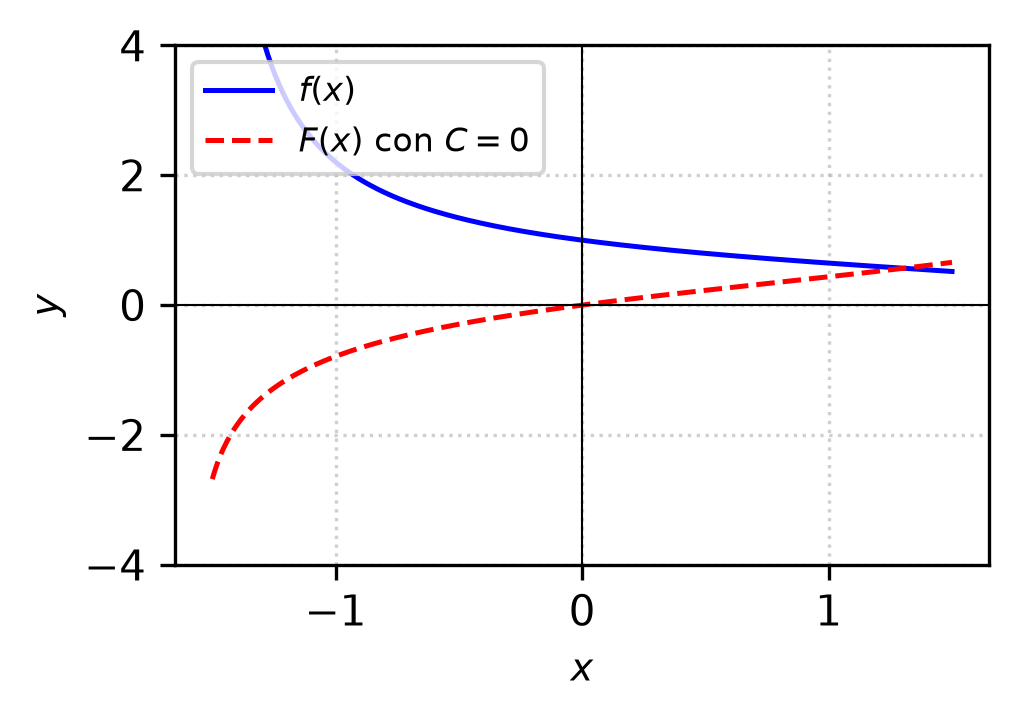
\includegraphics[width=\columnwidth]{semana_04/graficas/SEM04_P09_grafica.png}
	\caption{Representación gráfica de $f(x)$ y su antiderivada $F(x)$ evaluada para la constante de integración $C = 0$ (Problema 09).}
	\label{fig:problema09}
\end{figure}
